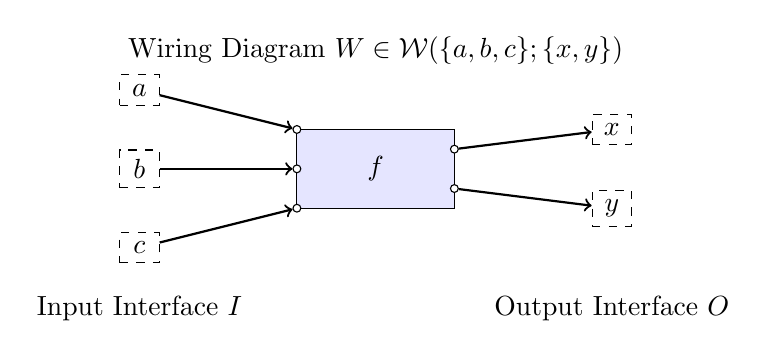
\begin{tikzpicture}[
  box/.style={rectangle, draw, minimum width=2cm, minimum height=1cm, fill=blue!10},
  wire/.style={->, thick},
  port/.style={circle, draw, fill=white, inner sep=1pt},
  interface/.style={rectangle, draw, dashed, minimum width=0.5cm, minimum height=0.3cm}
]

% Input interface
\node[interface] (in1) at (-3, 1) {$a$};
\node[interface] (in2) at (-3, 0) {$b$};
\node[interface] (in3) at (-3, -1) {$c$};

% Operation box
\node[box] (op1) at (0, 0) {$f$};

% Output interface  
\node[interface] (out1) at (3, 0.5) {$x$};
\node[interface] (out2) at (3, -0.5) {$y$};

% Input ports on box
\node[port] (p1) at (-1, 0.5) {};
\node[port] (p2) at (-1, 0) {};
\node[port] (p3) at (-1, -0.5) {};

% Output ports on box
\node[port] (q1) at (1, 0.25) {};
\node[port] (q2) at (1, -0.25) {};

% Wires
\draw[wire] (in1) -- (p1);
\draw[wire] (in2) -- (p2);
\draw[wire] (in3) -- (p3);
\draw[wire] (q1) -- (out1);
\draw[wire] (q2) -- (out2);

% Labels
\node[above] at (0, 1.2) {Wiring Diagram $W \in \mathcal{W}(\{a,b,c\}; \{x,y\})$};
\node[below] at (-3, -1.5) {Input Interface $I$};
\node[below] at (3, -1.5) {Output Interface $O$};

\end{tikzpicture}